\documentclass[preview]{standalone}

\usepackage[utf8]{inputenc}
\usepackage{amsmath, amssymb}
\usepackage{subcaption}
\usepackage{graphicx}

% Matplotlib2TikZ
\usepackage{pgfplots}

% Bold the 'Figure #' in the caption and separate it from the title/caption with a period
% Captions will be left justified
%\usepackage[aboveskip=1pt,labelfont=bf,labelsep=period,justification=raggedright,singlelinecheck=off]{caption}
\renewcommand{\figurename}{Fig}

%\captionsetup[figure]{labelfont=bf,textfont=bf,labelsep=period}

%\interfootnotelinepenalty=10000

\begin{document}
\begin{figure*}
	\centering
	\captionsetup[subfigure]{justification=centering}
	\begin{subfigure}{\textwidth}
% 	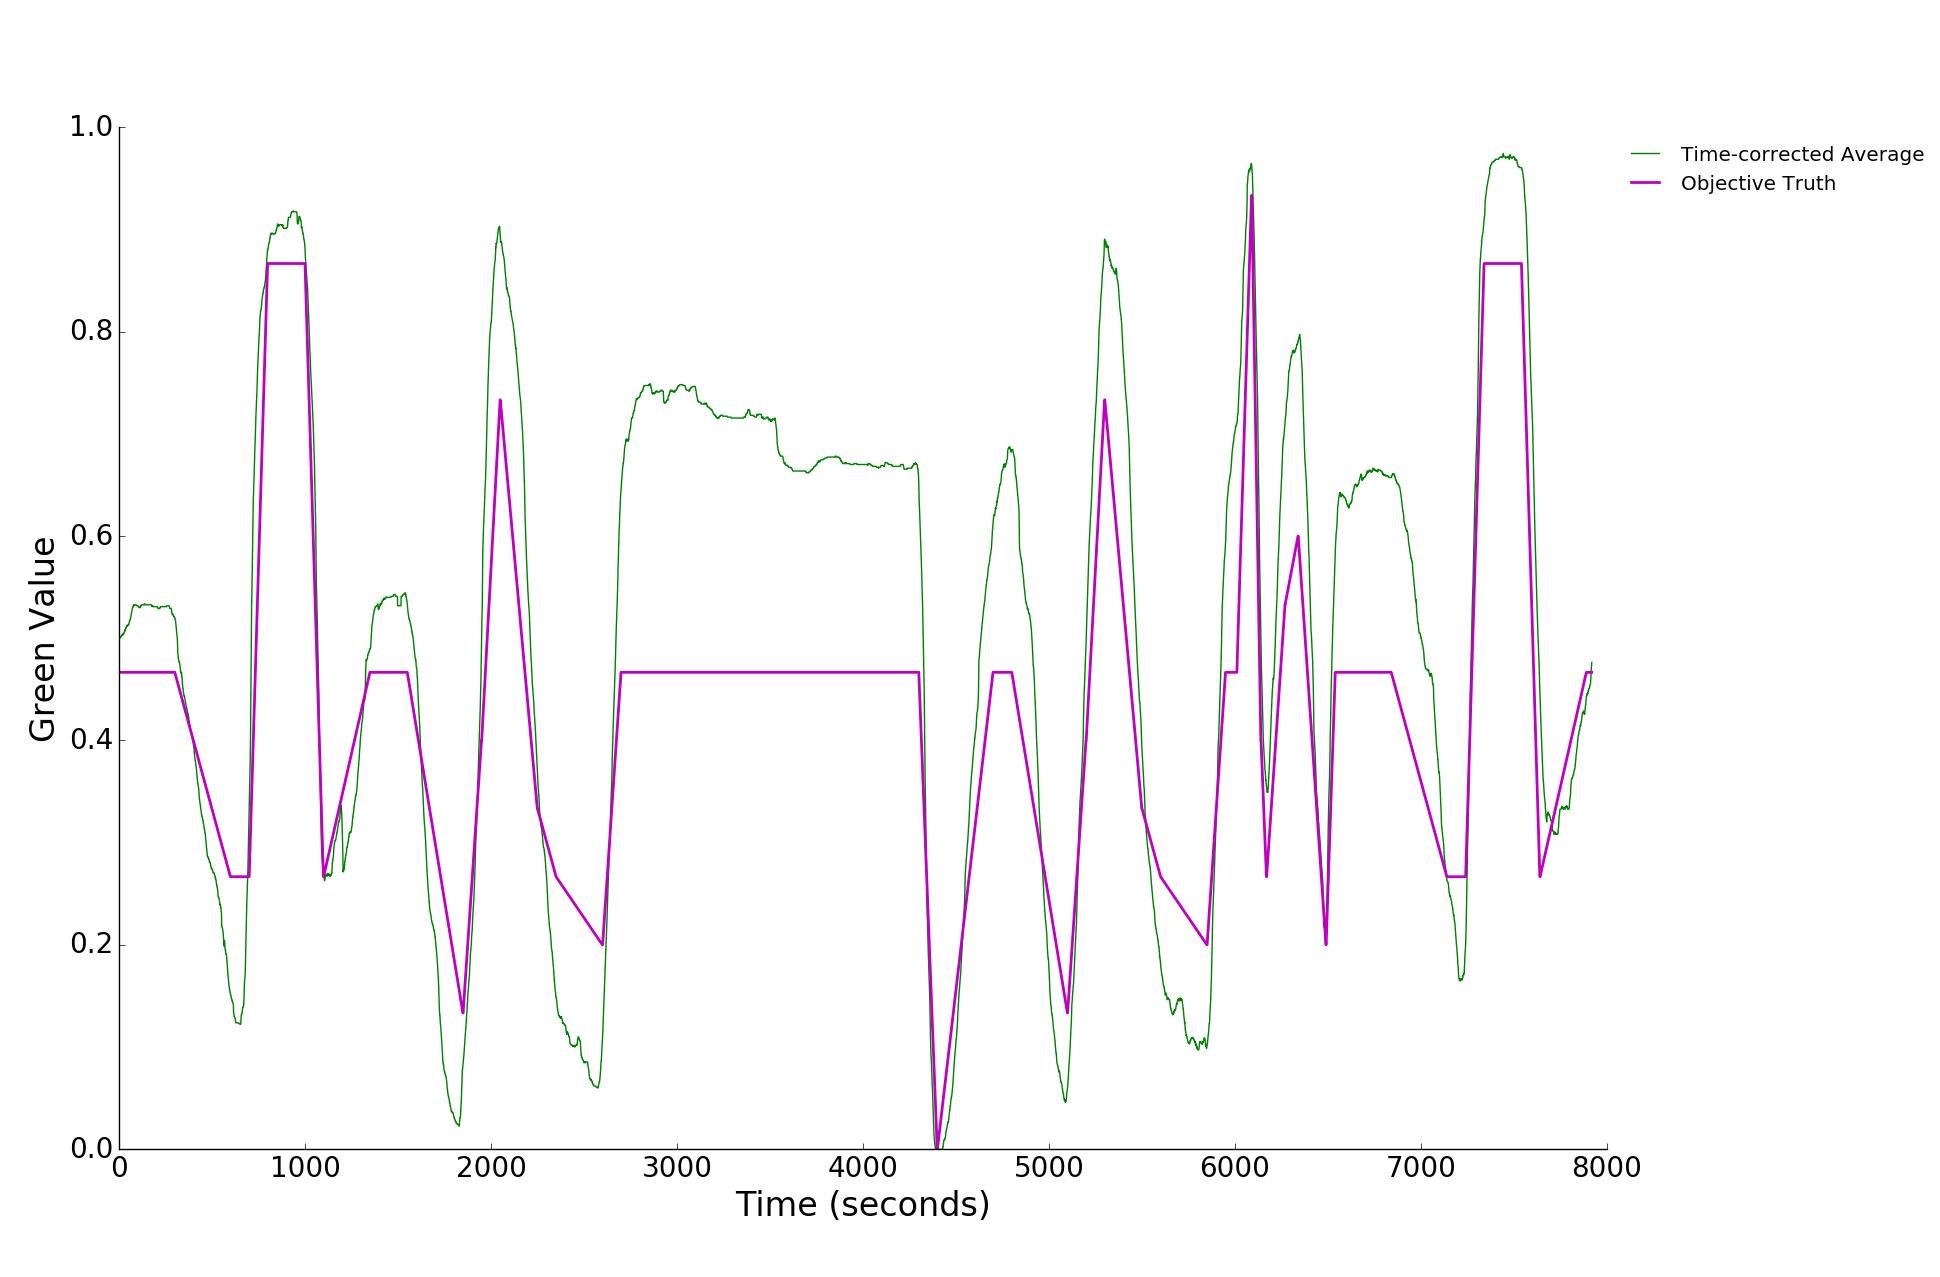
\includegraphics[width=\textwidth]{images/average_and_objective}
    \input{images/average_and_objective.tex}
%  	\vspace{-0.5cm}
 	\caption{Plot of time-corrected annotation average and objective truth.}
	\label{Fig:average_and_objective}
	\end{subfigure}
% 	\hfill
    
	\begin{subfigure}{\textwidth}
% 	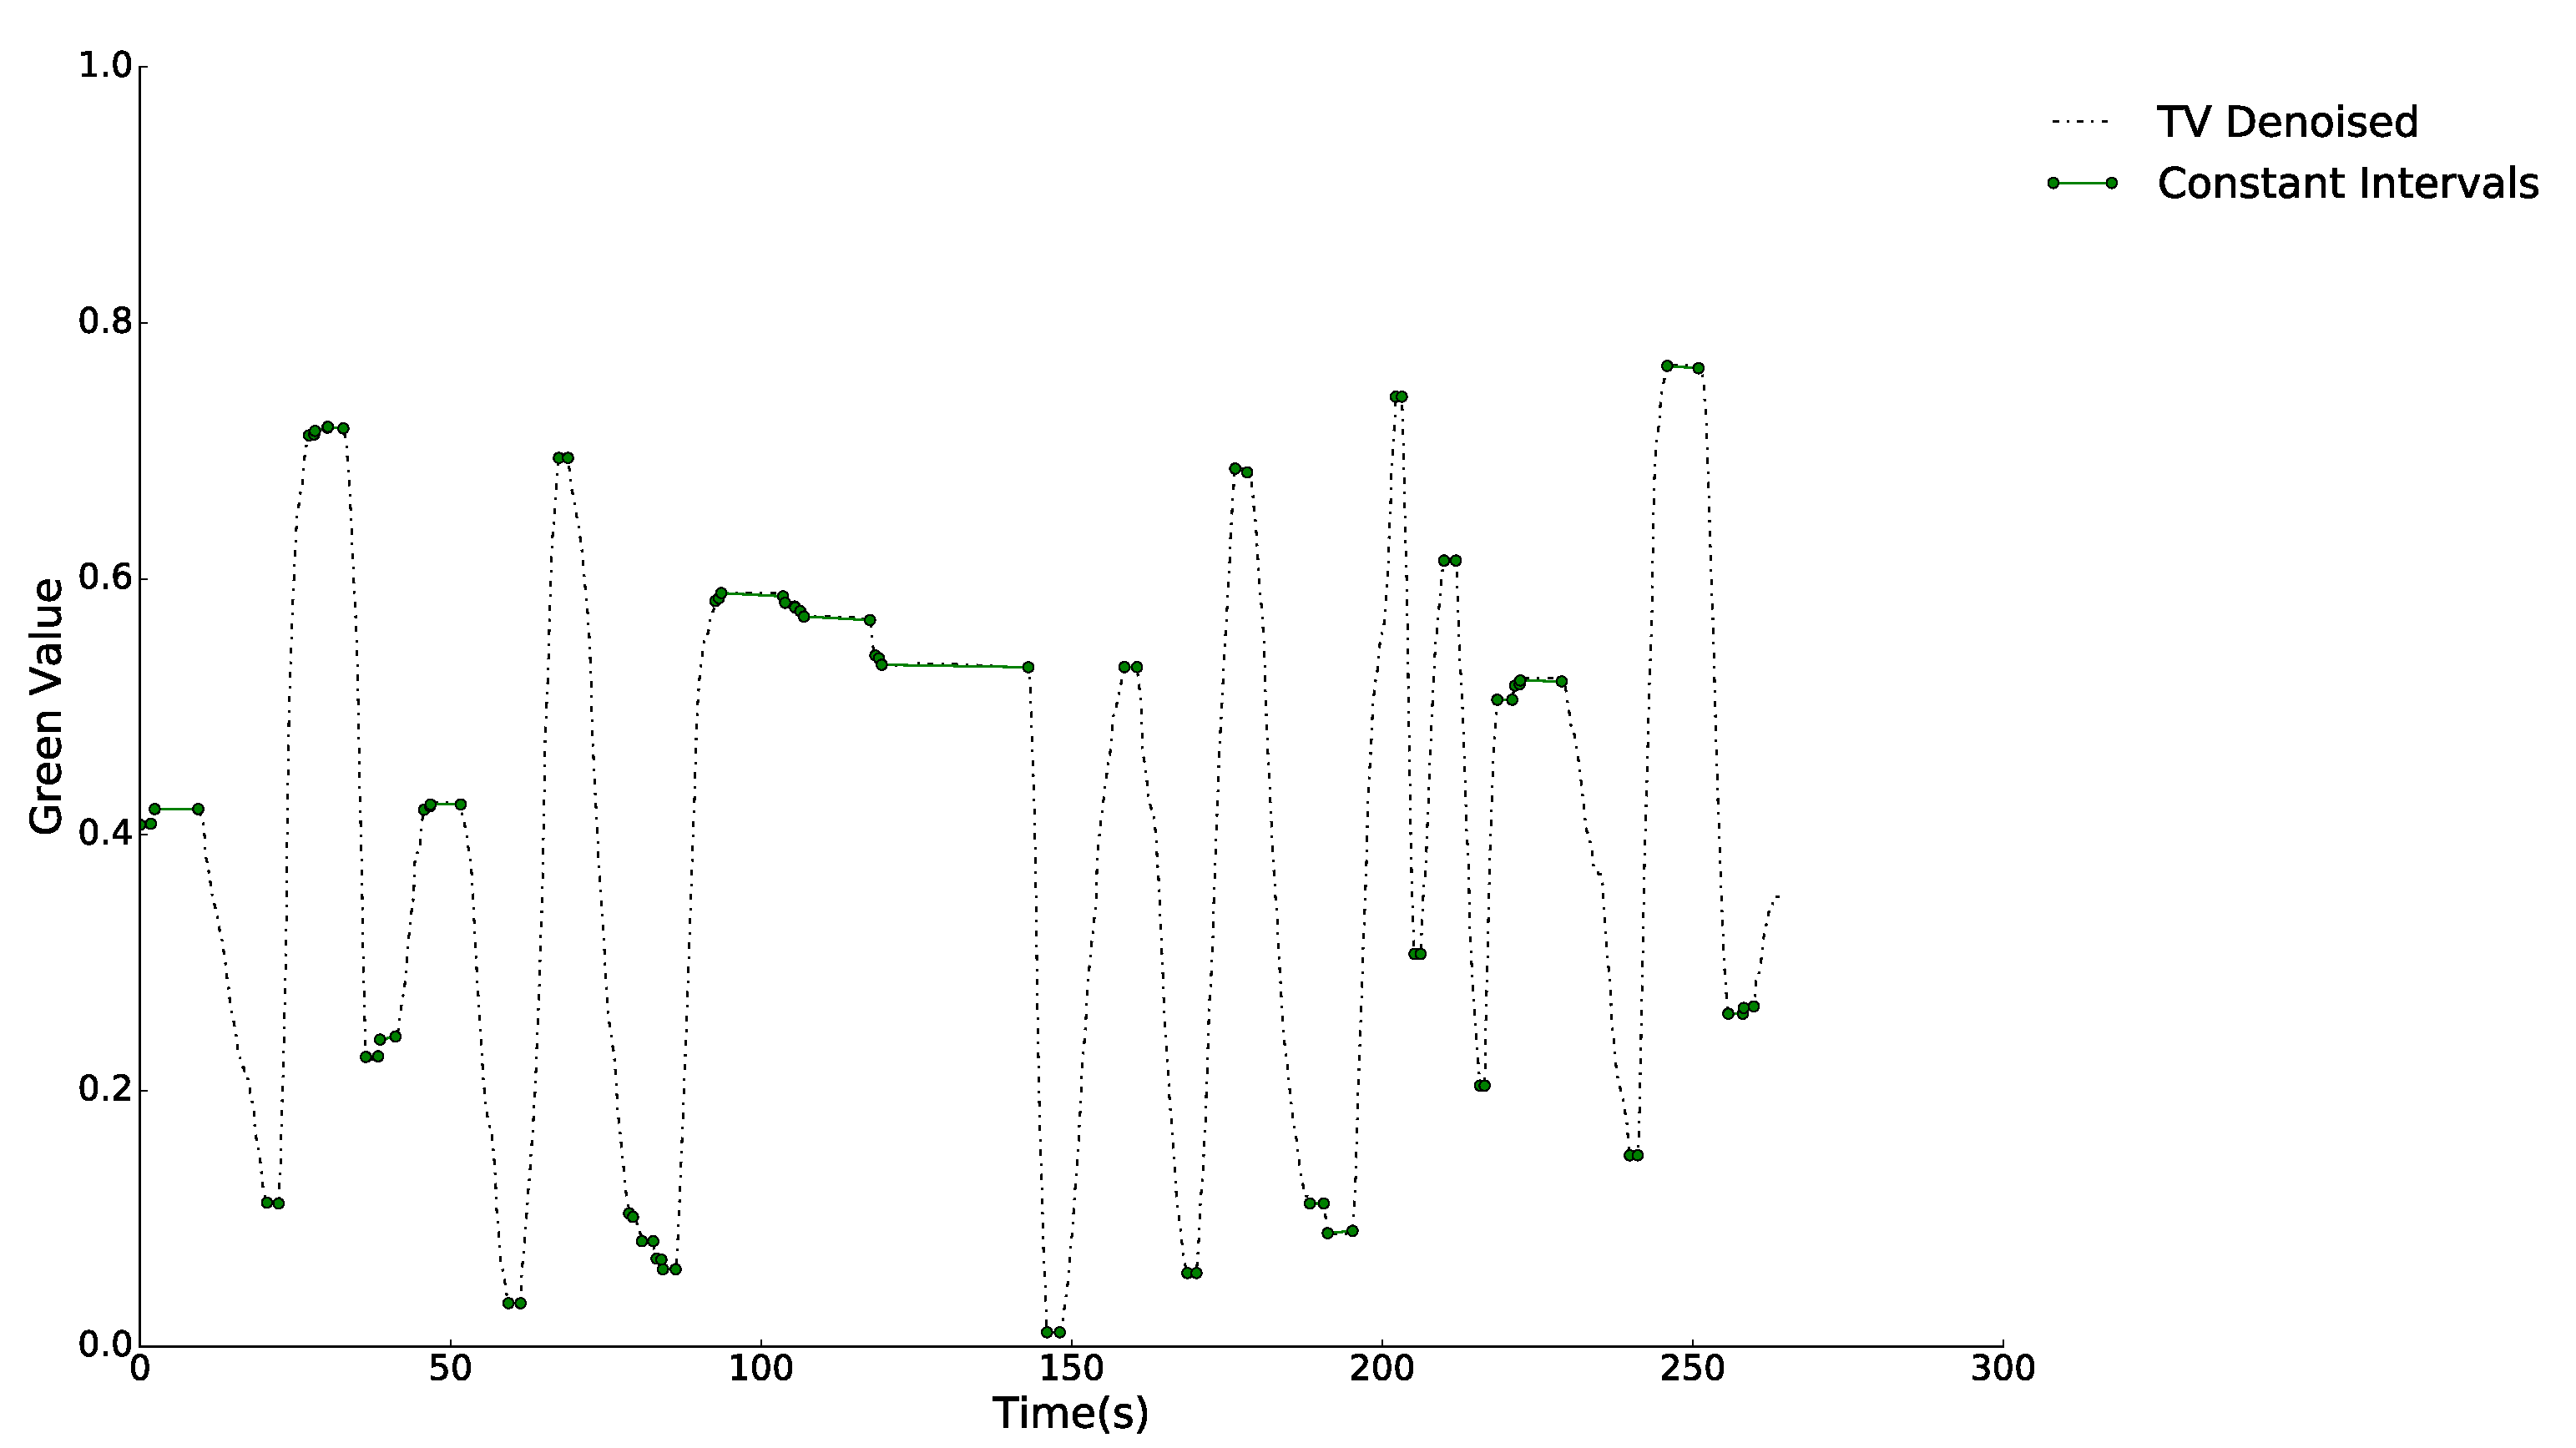
\includegraphics[width=\textwidth]{images/tv_and_intervals}
    \input{images/tv_and_intervals.tex}
% 	\vspace{-0.5cm}
	\caption{Plot of TV-denoised fused annotation with extracted constant intervals.}
	\label{Fig:tv_and_intervals}
	\end{subfigure}
\end{figure*}
\end{document}